% Practice Test 13 — Indiana Edition
% Questions: 30 (18 MC + 12 SA)
% Generated by scripts/generate_practice_tests.py

\begin{practiceQuestion}{1-3-q16}{mc}
\begin{questionText}
A map uses a scale where $1$ cm represents $25$ km. What is the constant of proportionality in km per cm?
\end{questionText}
\choiceA{$0.04$}
\choiceB{$1$}
\choiceC{$25$}
\choiceD{$250$}
\correctAnswer{C}
\explanation{$k = \frac{25 \text{ km}}{1 \text{ cm}} = 25$ km per cm.}
\end{practiceQuestion}

\begin{practiceQuestion}{1-5-q18}{mc}
\begin{questionText}
A store sells oranges. The graph passes through $(6, 4.50)$. What is the cost of $10$ oranges?
\end{questionText}
\choiceA{$\$6.50$}
\choiceB{$\$7.00$}
\choiceC{$\$7.50$}
\choiceD{$\$10.50$}
\correctAnswer{C}
\explanation{$k = \frac{4.50}{6} = 0.75$. Cost of $10$: $0.75 \times 10 = \$7.50$.}
\end{practiceQuestion}

\begin{practiceQuestion}{1-6-q14}{mc}
\begin{questionText}
A school orders $240$ lunches for $320$ students. At the same rate, how many lunches should they order for $400$ students?
\end{questionText}
\choiceA{$280$}
\choiceB{$300$}
\choiceC{$320$}
\choiceD{$360$}
\correctAnswer{B}
\explanation{$\frac{240}{320} = \frac{x}{400}$. Cross-multiply: $320x = 96{,}000$, so $x = 300$ lunches.}
\end{practiceQuestion}

\begin{practiceQuestion}{2-2-q19}{sa}
\begin{questionText}
Use a proportion to find $85\%$ of $260$.
\end{questionText}
\correctAnswer{$221$}
\explanation{$\frac{n}{260} = \frac{85}{100}$. Cross-multiply: $100n = 22{,}100$. Divide: $n = 221$.}
\end{practiceQuestion}

\begin{practiceQuestion}{2-5-q30}{gsa}
\begin{questionText}
The bar graph shows the monthly sales for a salesperson over $4$ months. She earns $6\%$ commission. What is her total commission for all $4$ months?

\begin{center}
\begin{tikzpicture}[scale=0.5]
  \draw[thick,->] (0,0) -- (0,7) node[above]{\small Sales (\$)};
  \draw[thick,->] (0,0) -- (9.5,0);
  \fill[funBlue!60] (0.5,0) rectangle (1.5,4);
  \fill[funBlue!60] (2.5,0) rectangle (3.5,5);
  \fill[funBlue!60] (4.5,0) rectangle (5.5,3);
  \fill[funBlue!60] (6.5,0) rectangle (7.5,6);
  \node[below,font=\small] at (1,0) {Jan};
  \node[below,font=\small] at (3,0) {Feb};
  \node[below,font=\small] at (5,0) {Mar};
  \node[below,font=\small] at (7,0) {Apr};
  \foreach \y/\lab in {2/4000,4/8000,6/12000} {
    \draw (-0.1,\y) -- (0.1,\y) node[left,font=\small,xshift=-2pt] {\lab};
  }
  \node[above,font=\small] at (1,4) {$8{,}000$};
  \node[above,font=\small] at (3,5) {$10{,}000$};
  \node[above,font=\small] at (5,3) {$6{,}000$};
  \node[above,font=\small] at (7,6) {$12{,}000$};
\end{tikzpicture}
\end{center}
\end{questionText}
\correctAnswer{$\$2{,}160$}
\explanation{Total sales: $8{,}000 + 10{,}000 + 6{,}000 + 12{,}000 = \$36{,}000$. Commission: $36{,}000 \times 0.06 = \$2{,}160$.}
\end{practiceQuestion}

\begin{practiceQuestion}{2-7-q22}{sa}
\begin{questionText}
A lab experiment expected to produce $250$ mL but produced $240$ mL. Find the percent error.
\end{questionText}
\correctAnswer{$\approx 4.2\%$}
\explanation{$\frac{|250 - 240|}{240} \times 100 = \frac{10}{240} \times 100 \approx 4.17 \approx 4.2\%$.}
\end{practiceQuestion}

\begin{practiceQuestion}{3-1-q01}{mc}
\begin{questionText}
What is the opposite of $-6$?
\end{questionText}
\choiceA{$-6$}
\choiceB{$0$}
\choiceC{$6$}
\choiceD{$\frac{1}{6}$}
\correctAnswer{C}
\explanation{The opposite of a negative number is positive. The opposite of $-6$ is $6$ because both are $6$ units from $0$.}
\end{practiceQuestion}

\begin{practiceQuestion}{3-2-q15}{mc}
\begin{questionText}
What is $(-25) + 13 + (-8)$?
\end{questionText}
\choiceA{$-20$}
\choiceB{$-46$}
\choiceC{$30$}
\choiceD{$-4$}
\correctAnswer{A}
\explanation{$(-25) + 13 = -12$. Then $(-12) + (-8) = -20$.}
\end{practiceQuestion}

\begin{practiceQuestion}{4-2-q21}{sa}
\begin{questionText}
Simplify $-2a + 5b + 7a - 3b$.
\end{questionText}
\correctAnswer{$5a + 2b$}
\explanation{Combine $a$-terms: $-2a + 7a = 5a$. Combine $b$-terms: $5b - 3b = 2b$. Result: $5a + 2b$.}
\end{practiceQuestion}

\begin{practiceQuestion}{4-3-q26}{gmc}
\begin{questionText}
The area model below represents a product. Which expression does it show?

\begin{center}
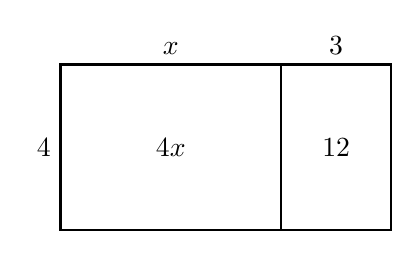
\begin{tikzpicture}[scale=0.7]
  % Outer rectangle
  \draw[thick] (0,0) rectangle (6,3);
  % Dividing line
  \draw[thick] (4,0) -- (4,3);
  % Labels
  \node[left] at (0,1.5) {$4$};
  \node[above] at (2,3) {$x$};
  \node[above] at (5,3) {$3$};
  % Inside labels
  \node at (2,1.5) {$4x$};
  \node at (5,1.5) {$12$};
\end{tikzpicture}
\end{center}
\end{questionText}
\choiceA{$4(x + 3) = 4x + 12$}
\choiceB{$4(x + 3) = 4x + 3$}
\choiceC{$3(x + 4) = 3x + 12$}
\choiceD{$(x + 3)(x + 4) = x^2 + 12$}
\correctAnswer{A}
\explanation{The height is $4$ and the width is split into $x$ and $3$. Multiply: $4 \times x = 4x$ and $4 \times 3 = 12$. So $4(x + 3) = 4x + 12$.}
\end{practiceQuestion}

\begin{practiceQuestion}{5-4-q06}{mc}
\begin{questionText}
Solve $-0.4y + 2 = 6$.
\end{questionText}
\choiceA{$y = 10$}
\choiceB{$y = -10$}
\choiceC{$y = 20$}
\choiceD{$y = -20$}
\correctAnswer{B}
\explanation{Subtract $2$: $-0.4y = 4$. Divide by $-0.4$: $y = -10$. Check: $-0.4(-10) + 2 = 4 + 2 = 6$ \checkmark.}
\end{practiceQuestion}

\begin{practiceQuestion}{5-5-q20}{sa}
\begin{questionText}
Solve $-5n + 10 \leq -15$.
\end{questionText}
\correctAnswer{$n \geq 5$}
\explanation{Subtract $10$: $-5n \leq -25$. Divide by $-5$ and flip: $n \geq 5$.}
\end{practiceQuestion}

\begin{practiceQuestion}{5-6-q16}{mc}
\begin{questionText}
Solve $\dfrac{x}{2} - 3 > 1$ and describe the graph.
\end{questionText}
\choiceA{Open circle at $8$, shade right}
\choiceB{Closed circle at $8$, shade right}
\choiceC{Open circle at $4$, shade right}
\choiceD{Open circle at $8$, shade left}
\correctAnswer{A}
\explanation{Add $3$: $\frac{x}{2} > 4$. Multiply by $2$: $x > 8$. Open circle at $8$, shade right.}
\end{practiceQuestion}

\begin{practiceQuestion}{6-1-q08}{mc}
\begin{questionText}
A scale drawing of a building uses $1$ in $= 10$ ft. The building is $85$ ft tall. How tall is it on the drawing?
\end{questionText}
\choiceA{$8$ in}
\choiceB{$8.5$ in}
\choiceC{$85$ in}
\choiceD{$850$ in}
\correctAnswer{B}
\explanation{Divide actual length by the scale factor: $85 \div 10 = 8.5$ in.}
\end{practiceQuestion}

\begin{practiceQuestion}{6-3-q23}{sa}
\begin{questionText}
Can a quadrilateral have sides $1$, $1$, $1$, and $10$?
\end{questionText}
\correctAnswer{No}
\explanation{For a quadrilateral, the longest side must be less than the sum of the other three. Here $1 + 1 + 1 = 3 < 10$, so it is impossible.}
\end{practiceQuestion}

\begin{practiceQuestion}{6-4-q12}{mc}
\begin{questionText}
Given angles $30°$ and $110°$ and the included side $6$ cm, how many triangles can be drawn?
\end{questionText}
\choiceA{None, because $30 + 110 > 180$}
\choiceB{None, because the third angle would be negative}
\choiceC{Exactly one}
\choiceD{Infinitely many}
\correctAnswer{C}
\explanation{$30 + 110 = 140°$. Third angle: $180° - 140° = 40°$. ASA produces one unique triangle.}
\end{practiceQuestion}

\begin{practiceQuestion}{6-5-q09}{mc}
\begin{questionText}
You cut a cone with a vertical slice through its apex (tip). What shape is the cross-section?
\end{questionText}
\choiceA{Circle}
\choiceB{Triangle}
\choiceC{Rectangle}
\choiceD{Semicircle}
\correctAnswer{B}
\explanation{A vertical cut through the apex of a cone produces a triangle (specifically an isosceles triangle).}
\end{practiceQuestion}

\begin{practiceQuestion}{6-6-q14}{mc}
\begin{questionText}
Angles $A$ and $B$ are complementary. Angle $A$ is $(3x - 5)°$ and angle $B$ is $(x + 15)°$. What is angle $A$?
\end{questionText}
\choiceA{$20°$}
\choiceB{$35°$}
\choiceC{$55°$}
\choiceD{$65°$}
\correctAnswer{C}
\explanation{$3x - 5 + x + 15 = 90$. Combine: $4x + 10 = 90$. Solve: $4x = 80$, $x = 20$. Angle $A$: $3(20) - 5 = 55°$.}
\end{practiceQuestion}

\begin{practiceQuestion}{6-7-q27}{gmc}
\begin{questionText}
Point $T$ is shown on the coordinate plane. It is translated right $3$ and up $4$. Where is $T'$?

\begin{center}
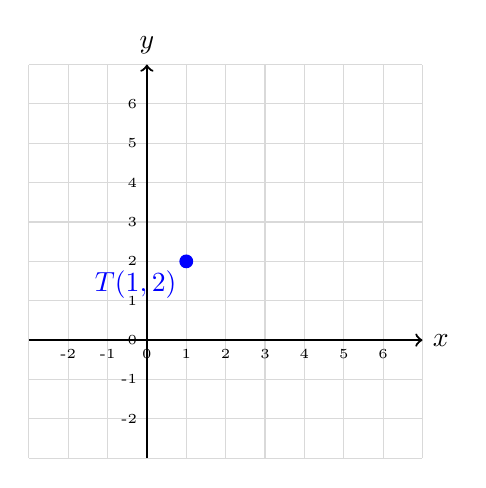
\begin{tikzpicture}[scale=0.5]
  \draw[step=1,gray!30,thin] (-3,-3) grid (7,7);
  \draw[thick,->] (-3,0) -- (7,0) node[right]{$x$};
  \draw[thick,->] (0,-3) -- (0,7) node[above]{$y$};
  \fill[blue] (1,2) circle (5pt);
  \node[below left,blue] at (1,2) {$T(1,2)$};
  \foreach \x in {-2,...,6} \node[below,font=\tiny] at (\x,0) {\x};
  \foreach \y in {-2,...,6} \node[left,font=\tiny] at (0,\y) {\y};
\end{tikzpicture}
\end{center}
\end{questionText}
\choiceA{$(4, 6)$}
\choiceB{$(4, -2)$}
\choiceC{$(-2, 6)$}
\choiceD{$(1, 6)$}
\correctAnswer{A}
\explanation{Right $3$: $1 + 3 = 4$. Up $4$: $2 + 4 = 6$. So $T'(4, 6)$.}
\end{practiceQuestion}

\begin{practiceQuestion}{7-3-q08}{mc}
\begin{questionText}
A circle has an area of $50.24$ m$^2$. Using $\pi \approx 3.14$, what is the diameter?
\end{questionText}
\choiceA{$4$ m}
\choiceB{$8$ m}
\choiceC{$16$ m}
\choiceD{$2$ m}
\correctAnswer{B}
\explanation{$r^2 = 50.24 \div 3.14 = 16$. So $r = 4$ m and $d = 8$ m.}
\end{practiceQuestion}

\begin{practiceQuestion}{7-4-q20}{sa}
\begin{questionText}
A figure is a rectangle $15$ m by $8$ m with a rectangular hole $5$ m by $3$ m cut out. What is the area of the remaining figure?
\end{questionText}
\correctAnswer{$105$ m$^2$}
\explanation{Outer: $15 \times 8 = 120$ m$^2$. Hole: $5 \times 3 = 15$ m$^2$. Remaining: $120 - 15 = 105$ m$^2$.}
\end{practiceQuestion}

\begin{practiceQuestion}{7-5-q19}{sa}
\begin{questionText}
Find the surface area of a rectangular prism with length $8$ cm, width $5$ cm, and height $3$ cm.
\end{questionText}
\correctAnswer{$158$ cm$^2$}
\explanation{$SA = 2(8 \times 5) + 2(8 \times 3) + 2(5 \times 3) = 80 + 48 + 30 = 158$ cm$^2$.}
\end{practiceQuestion}

\begin{practiceQuestion}{7-6-q29}{gsa}
\begin{questionText}
A composite solid is made of two rectangular prisms joined together as shown. What is the total volume?

\begin{center}
\begin{tikzpicture}[scale=0.35]
  % Bottom prism
  \draw[thick,funBlue,fill=funBlue!10] (0,0) rectangle (10,3);
  \draw[thick,funBlue,fill=funBlue!20] (10,0) -- (13,2) -- (13,5) -- (10,3) -- cycle;
  \draw[thick,funBlue,fill=funBlue!15] (0,3) -- (3,5) -- (13,5) -- (10,3) -- cycle;
  % Top prism
  \draw[thick,funRed,fill=funRed!10] (0,3) rectangle (4,6);
  \draw[thick,funRed,fill=funRed!20] (4,3) -- (7,5) -- (7,8) -- (4,6) -- cycle;
  \draw[thick,funRed,fill=funRed!15] (0,6) -- (3,8) -- (7,8) -- (4,6) -- cycle;
  % Labels
  \node[below] at (5,0) {$10$ cm};
  \node[left] at (0,1.5) {$3$ cm};
  \node[right] at (13,3.5) {$3$ cm};
  \node[left] at (0,4.5) {$3$ cm};
  \node[above left] at (2,6) {$4$ cm};
  \node[right] at (7,6.5) {$3$ cm};
\end{tikzpicture}
\end{center}
\end{questionText}
\correctAnswer{$126$ cm$^3$}
\explanation{Bottom prism: $10 \times 3 \times 3 = 90$ cm$^3$. Top prism: $4 \times 3 \times 3 = 36$ cm$^3$. Total: $90 + 36 = 126$ cm$^3$.}
\end{practiceQuestion}

\begin{practiceQuestion}{8-1-q23}{sa}
\begin{questionText}
A radio station asks listeners to call in and vote for their favorite song. Explain why this is not a random sample.
\end{questionText}
\correctAnswer{Only listeners who choose to call participate, so it is voluntary and biased}
\explanation{Voluntary response samples are biased because people with strong opinions are more likely to respond.}
\end{practiceQuestion}

\begin{practiceQuestion}{8-3-q15}{mc}
\begin{questionText}
Group X: mean $45$, range $12$. Group Y: mean $52$, range $12$. What can you say about these groups?
\end{questionText}
\choiceA{They have the same center and different spread}
\choiceB{They have different centers and the same spread}
\choiceC{They are identical}
\choiceD{Group X is more spread out}
\correctAnswer{B}
\explanation{The means differ ($45$ vs.\ $52$) but both have the same range ($12$), so they have different centers and similar spread.}
\end{practiceQuestion}

\begin{practiceQuestion}{8-4-q20}{sa}
\begin{questionText}
Data: $8, 10, 12, 14, 16, 18, 20$. Find the IQR.
\end{questionText}
\correctAnswer{$8$}
\explanation{$Q_1 = 10$, $Q_3 = 18$. IQR $= 18 - 10 = 8$.}
\end{practiceQuestion}

\begin{practiceQuestion}{8-7-q24}{sa}
\begin{questionText}
Give one advantage and one disadvantage of using a frequency table compared to a bar graph.
\end{questionText}
\correctAnswer{Advantage: shows exact counts; Disadvantage: harder to see trends or compare visually}
\explanation{Tables give precise numbers but graphs make patterns and comparisons easier to spots at a glance.}
\end{practiceQuestion}

\begin{practiceQuestion}{9-4-q18}{mc}
\begin{questionText}
Ben predicts that a coin will land on heads $50\%$ of the time. He flips the coin $20$ times and gets $14$ heads. What should he conclude?
\end{questionText}
\choiceA{The coin is definitely biased}
\choiceB{His model is exactly correct}
\choiceC{The result is somewhat different from the prediction, but $20$ trials is a small sample}
\choiceD{He should change his model to predict $70\%$ heads}
\correctAnswer{C}
\explanation{$\frac{14}{20} = 0.70$ vs. predicted $0.50$. With only $20$ trials, variation is expected. More trials would provide a better comparison.}
\end{practiceQuestion}

\begin{practiceQuestion}{9-6-q28}{gmc}
\begin{questionText}
The table below shows the sample space for spinning two spinners. Spinner 1 has sections $\{1, 2, 3\}$ and Spinner 2 has sections $\{A, B\}$. If each outcome is equally likely, what is the probability of getting an odd number and the letter B?

\begin{center}
\begin{tabular}{|c|c|c|}
\hline
 & \textbf{A} & \textbf{B} \\
\hline
\textbf{1} & $(1,A)$ & \cellcolor{funGreen!20}$(1,B)$ \\
\hline
\textbf{2} & $(2,A)$ & $(2,B)$ \\
\hline
\textbf{3} & $(3,A)$ & \cellcolor{funGreen!20}$(3,B)$ \\
\hline
\end{tabular}
\end{center}
\end{questionText}
\choiceA{$\frac{1}{6}$}
\choiceB{$\frac{2}{6}$}
\choiceC{$\frac{3}{6}$}
\choiceD{$\frac{4}{6}$}
\correctAnswer{B}
\explanation{Odd numbers: $1, 3$. Favorable outcomes: $(1,B)$ and $(3,B)$ — $2$ out of $6$. $P = \frac{2}{6} = \frac{1}{3}$.}
\end{practiceQuestion}

\begin{practiceQuestion}{9-7-q02}{mc}
\begin{questionText}
A coin flip is used to simulate an event with two equally likely outcomes. Which real-world event could it model?
\end{questionText}
\choiceA{The probability of rain ($30\%$ chance)}
\choiceB{Whether a baby is a boy or girl (approximately $50\%$ each)}
\choiceC{Rolling a $6$ on a die}
\choiceD{Drawing a heart from a deck of cards}
\correctAnswer{B}
\explanation{A coin has two equally likely outcomes ($50\%$ each), which matches the approximately $50/50$ chance of a baby being a boy or girl.}
\end{practiceQuestion}
